\clearpage
\chapter{Analytical Problem 3.3: Least Squares IIR Identification}

Wir kennen das IIR-System $u[n] = v[n] + u[n-1] - \frac{1}{8} u[n-2]$, von dem $M$ Input-Output-Samples vorhanden sind.
F�r die folgende Differenzengleichung sollen die Parameter $a_k$ und $b_k$ bestimmt werden, wobei die Anzahl der Parameter $N = N_a + N_b + 1$ ist und $M \geq N$ ist:

\begin{equation}
  u[n] = \sum_{k=0}^{N_b} b_k v[n-k] - \sum_{k=1}^{N_a} a_k u[n-k]
\end{equation}


\paragraph{a)}

Es soll eine LS-L�sung (\emph{least squares}) f�r die Parameter gefunden werden.

Dazu wird zun�chst ein Parametervektor $\mathbf{c} = \begin{bmatrix} \mathbf{b} \\ - \mathbf{a} \end{bmatrix}$ eingef�hrt.

Weiters muss ein \emph{tap input/output vector} $\mathbf{x}[n] = \begin{bmatrix} \mathbf{v}[n] \\ \mathbf{u}[n] \end{bmatrix}$ eingef�hrt werden, mit $\mathbf{v}[n] = \begin{bmatrix} v[n-0] \\ v[n-1] \\ \vdots \\ v[n - N_b] \end{bmatrix}$ und $\mathbf{u}[n] = \begin{bmatrix} u[n-1] \\ u[n-2] \\ \vdots \\ u[n - N_a] \end{bmatrix}$.

F�r die LS-Solution gehen wir nun wie gewohnt vor. Der quadratische Fehler soll minimiert werden ($e[n]$ ist der Fehler, $d[n]$ das gew�nschte Signal). Dazu wird eine einfache Gleichung aufgestellt und in Vektorschreibweise �bergef�hrt:

\begin{equation}
  e[n] = d[n] - y[n] = d[n] - \mathbf{c}^T \mathbf{x}[n] = d[n] - \mathbf{x}^T[n] \mathbf{c} \;\; \Rightarrow \mathbf{e} = \mathbf{d} - \mathbf{X} \mathbf{c}
\end{equation}

$\mathbf{X}$ ist die Designmatrix mit folgender Struktur:

\begin{equation}
  \mathbf{X} = \begin{bmatrix} \mathbf{x}^T[0] \\ \mathbf{x}^T[1] \\ \vdots \\ \mathbf{x}^T[M] \end{bmatrix}
\end{equation}

Jetzt bestimmen wir die LS-Solution wie gehabt:

\begin{eqnarray}
  J(\mathbf{c}) & = & \sum_{n=0}^{M} \left| e[n] \right|^2 = \left| \left| \mathbf{e} \right| \right|^2 = \langle \mathbf{e}, \mathbf{e} \rangle = \mathbf{e}^T \mathbf{e} = (\mathbf{d} - \mathbf{X} \mathbf{c})^T (\mathbf{d} - \mathbf{X} \mathbf{c}) = (\mathbf{d}^T - \mathbf{c}^T \mathbf{X}^T) (\mathbf{d} - \mathbf{X} \mathbf{c}) \\
  & = & \mathbf{d}^T \mathbf{d} - \mathbf{d}^T \mathbf{X} \mathbf{c} - \underbrace{\mathbf{c}^T \mathbf{X}^T \mathbf{d}}_{\mathbf{d}^T \mathbf{X} \mathbf{c}} + \mathbf{c}^T \mathbf{X}^T \mathbf{X} \mathbf{c} = \mathbf{d}^T \mathbf{d} - 2 \mathbf{d}^T \mathbf{X} \mathbf{c} + \mathbf{c}^T \mathbf{X}^T \mathbf{X} \mathbf{c}
\end{eqnarray}

Die L�sung ergibt sich durch Ableiten und Null setzen der Kostenfunktion:

\begin{eqnarray}
  \mathbf{\triangledown}_{\mathbf{c}} J(\mathbf{c}) & = & 0 - 2 \mathbf{d}^T \mathbf{X} + 2 \mathbf{c}^T \mathbf{X}^T \mathbf{X} \stackrel{!}{=} 0 \\
  & \Rightarrow & \mathbf{d}^T \mathbf{X} \stackrel{!}{=} \mathbf{c}^T \mathbf{X}^T \mathbf{X} \\
  & \Rightarrow & \mathbf{X}^T \mathbf{d} \stackrel{!}{=} \mathbf{X}^T \mathbf{X}^T \mathbf{c} \\
  & & \Rightarrow \mathbf{c}_{LS} = (\mathbf{X}^T \mathbf{X})^{-1} \mathbf{X}^T \mathbf{d}
\end{eqnarray}

Aus dieser L�sung kann man die Parameter $\{ a_k \}$ und $\{b_k\}$ ablesen (siehe oben).

Diese L�sung entspricht der LS-Solution f�r FIR-Filter! $\mathbf{X}$ und $\mathbf{d}$ haben jedoch wie oben beschrieben eine spezielle Form \footnote{f�r die nicht vorhandenen Werte (z.B. $v[-1]$) wird 0 eingesetzt.}:

\begin{equation}
  \mathbf{X} = \begin{bmatrix} \mathbf{x}^T[0] \\ \mathbf{x}^T[1] \\ \vdots \\ \mathbf{x}^T[M] \end{bmatrix}
  = \begin{bmatrix} v[0] & v[-1] & v[-2] & \cdots & v[-N_b] & u[-1] & u[-2] & \cdots & u[-N_a] \\
                    v[1] & v[0] & v[-1] & \cdots & v[-(N_b+1)] & u[0] & u[-1] & \cdots & u[-(N_a+1)] \\
                    v[2] & v[1] & v[0] & \cdots & v[-(N_b+2)] & u[1] & u[0] & \cdots & u[-(N_a+2)] \\
                    \vdots & \ddots \end{bmatrix}
\end{equation}

Das gew�nschte Signal $d[n]$ entspricht dem Ausgangssignal des IIR-Filters:

\begin{equation}
  d[n] = v[n] + d[n-1] - \frac{1}{8} d[n-2] \;\; \Rightarrow \mathbf{d} = \begin{bmatrix} v[0] + 0 - \frac{1}{8} 0 \\ v[1] + v[0] - \frac{1}{8} 0 \\ v[2] + (v[1] + v[0]) - \frac{1}{8} v[0] \\ v[3] + (v[2] + v[1] + v[0] - \frac{1}{8} v[0]) - \frac{1}{8} (v[1] + v[0]) \\ \vdots \end{bmatrix}
\end{equation}


\paragraph{b)}

Nun soll f�r die Eingangsfolge $\{v[n]\} = \{1, 0, 0\}$ die Ausgangsfolge $\{u[n]\}$ berechnet werden. F�r die Anzahl der Parameter gilt $N_a = 1, N_b = 0$, es gibt also nur 2 Parameter: $a_1$ und $b_0$.

Wir evaluieren nun die Differenzengleichung f�r ein paar Iterationen (die Werte werden sp�ter ben�tigt):

\begin{eqnarray}
  u[n] & = & v[n] + u[n-1] - \frac{1}{8} u[n-2] \\
  \Rightarrow u[0] & = & v[0] + u[-1] - \frac{1}{8} u[-2] = v[0] + 0 - \frac{1}{8} 0 = v[0] = 1 \\
  u[1] & = & v[1] + u[0] - \frac{1}{8} u[-1] = 1 \\
  u[2] & = & v[2] + u[1] - \frac{1}{8} u[0] = 0 + 1 - \frac{1}{8} 1 = \frac{7}{8} \\
  u[3] & = & v[3] + u[2] - \frac{1}{8} u[1] = 0 + \frac{7}{8} - \frac{1}{8} 1 = \frac{3}{4} \\
  u[4] & = & v[4] + u[3] - \frac{1}{8} u[2] = 0 + \frac{3}{4} - \frac{1}{8} \frac{7}{8} = \frac{41}{64} \\
  u[5] & = & v[5] + u[4] - \frac{1}{8} u[3] = 0 + \frac{41}{64} - \frac{1}{8} \frac{3}{4} = \frac{35}{64} \\
  \vdots
\end{eqnarray}

Mit diesen berechneten Werten kann man nun die Matrix $\mathbf{X}$ und den Vektor $\mathbf{d}$ aufstellen (f�r die vorher berechneten 5 Iterationen):

\begin{equation}
  \mathbf{X} = \begin{bmatrix} v[0] & u[-1] \\ v[1] & u[0] \\ v[2] & u[1] \\ v[3] & u[2] \\ v[4] & u[3] \\ v[5] & u[4] \end{bmatrix} = 
  \begin{bmatrix} 1 & 0 \\ 0 & 1 \\ 0 & 1 \\ 0 & \frac{7}{8} \\ 0 & \frac{3}{4} \\ 0 & \frac{41}{64} \end{bmatrix},
  \;\;\;
  \mathbf{d} = \begin{bmatrix} u[0] \\ u[1] \\ u[2] \\ u[3] \\ u[4] \\ u[5] \end{bmatrix} = 
  \begin{bmatrix} 1 \\ 1 \\ \frac{7}{8} \\ \frac{3}{4} \\ \frac{41}{64} \\ \frac{35}{64} \end{bmatrix}
\end{equation}

Mit der oben aufgestellten Formel f�r $\mathbf{c}_{LS}$ berechnen wir nun die Parameter $a_1$ und $b_0$ (in Matlab):

\begin{equation}
  \mathbf{c}_{LS} = (\mathbf{X}^T \mathbf{X})^{-1} \mathbf{X}^T \mathbf{d} \stackrel{Matlab}{=} \begin{bmatrix} 1 \\ 0.8993 \end{bmatrix} \; \Rightarrow b_0 = 1, a_1 = -0.8993
\end{equation}


\paragraph{c)}

Verglichen mit dem Modell aus Problem 3.1 mit N=1 stimmen die Parameter gut �berein. Im Problem 3.3 kommt es jedoch stark darauf an, wie viele Iterationen f�r die Berechnung von $\mathbf{c}_{LS}$ verwendet werden. Je mehr Iterationen, desto genauer wird das Ergebnis (desto genauer kommt es an das Ergebnis von Problem 3.1 heran). Das liegt in der Natur des IIR-Filters, da es sehr lange dauert, bis die Ausgangswerte des IIR-Filters auf vernachl�ssigbar kleine Werte gesunken sind.

Zur Bestimmung der Frequence response bringen wir die Differenzengleichung zuerst in den z-Bereich:

\begin{equation}
  u[n] = b_0 v[n] - a_1 u[n-1] \;\; \Leftrightarrow \;\; U(z) = b_0 V(z) - a_1 U(z) z^{-1}
\end{equation}

Nun stellen wir die �bertragungsfunktion $H(z)$ auf:

\begin{equation}
  H(z) = \frac{U(z)}{V(z)} = \frac{b_0}{1 + a_1 z^{-1}} = b_0 \frac{z}{z + a_1}
\end{equation}

Mit dem Befehl \texttt{freqz} kann man in Matlab die Frequency response dieses Systems plotten. Das Ergebnis ist in Abbildung~\ref{fig:3_3_c_freqresponse} dargestellt.

\begin{figure}[h!]
  \centering
  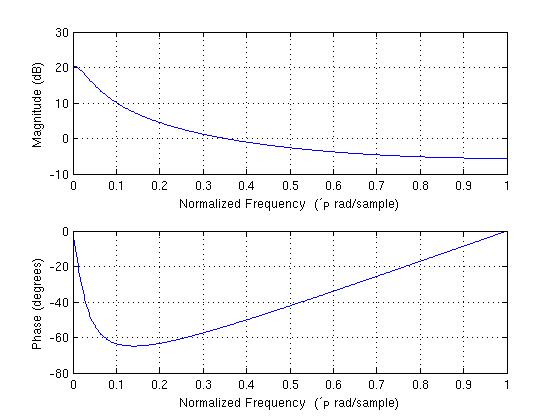
\includegraphics[width=0.7\textwidth]{./plots/3_3_c_freqresponse.png}
  % 3_3_c_freqresponse.png: 560x420 pixel, 90dpi, 15.81x11.85 cm, bb=0 0 448 336
  \caption{Frequency response des Systems aus Problem 3.3}
  \label{fig:3_3_c_freqresponse}
\end{figure}

\begin{LARGE}TODO\end{LARGE} Die Frequency response stimmt gut mit der von Problem 3.1 �berein. Man erkennt die �hnlichkeit der beiden Probleme.

Bei der R�cktransformation der �bertragungsfunktion aus dem z-Bereich ergibt sich f�r die Impulsantwort (mit Hilfe einer Transformationstabelle):

\begin{equation}
  h[n] = b_0 \cdot (-a_1)^n
\end{equation}

Daraus kann der Noise Gain berechnet werden:

\begin{equation}
  NG = \left|\left| \mathbf{h} \right| \right|^2 = \sum_{n=0}^{\infty} (b_0 (-a_1)^n)^2 = b_0^2 \sum_{n=0}^{\infty} (-a_1)^{2n} = 1^2 \sum_{n=0}^{\infty} (0.8993)^{2n} = \sum_{n=0}^{\infty} (0.8993^2)^n = \frac{1}{1 - 0.8993^2} = 5.23
\end{equation}

Dieser ist auch wieder h�her als bei Problem 3.1, nimmt aber mit steigender Anzahl von ber�cksichtigten Iterationen ab.
